\documentclass[letterpaper,12pt]{article}
\usepackage{fullpage}
\usepackage{fancyvrb,fancyhdr}
\usepackage{amsfonts}
\usepackage{array}
\usepackage{multirow}
\usepackage{amsmath, amssymb, amsthm}
\usepackage{graphicx,longtable, booktabs}
\usepackage[flushleft]{threeparttable}
\usepackage[footnotesize,center]{subfigure}
\usepackage{enumerate}
\usepackage{lastpage}
\usepackage{url}
\usepackage{mathrsfs}
\usepackage{cancel}
\usepackage{cite}
\usepackage{soul}
\usepackage{MnSymbol}
% Pseudo Code
\usepackage{algorithm}
\usepackage{algorithmic}
% Comments are in red
\usepackage{color}

\oddsidemargin 0in \evensidemargin 0in
\topmargin -0.5in \headheight 0.25in \headsep 0.25in
\textwidth 6.5in \textheight 9in %\marginparsep 0pt \marginparwidth 0pt
\parskip 0ex \parindent 10pt \footskip 20pt

\newfont{\bssten}{cmssbx10}
\newfont{\bssnine}{cmssbx10 scaled 900}
\newfont{\bssdoz}{cmssbx10 scaled 1200}

\pagestyle{fancy}
\fancyhead[LO]{\bssnine Diabetic Retinopathy}
% \fancyhead[R]{} \fancyhead[LO]{}
\fancyhead[RO]{\bssnine \thepage/\pageref{LastPage}}
%\fancyhead[RO]{\thepage}
\lfoot{} \cfoot{} \rfoot{}

%\usepackage[pdftex]{hyperref}

\def\t#1{{\tt #1}}
\newfont{\sserifn}{cmssbx10 at 11pt}
\newfont{\sserifo}{cmssbx10 at 12pt}

% Defining new \vect{} command to use a bold letter as a vector
\newcommand{\vect}[1]{\mathbf{#1}}
\newcommand{\erfc}{\mathrm{erfc}}
\newcommand{\figref}[1]{Figure~\ref{#1}}
\newcommand{\tableref}[1]{Table~\ref{#1}}
\newcommand{\eqsref}[1]{Eq.~\ref{#1}}
\newcommand{\algref}[1]{Algorithm~\ref{#1}}

%opening                    

\usepackage[para,multiple]{footmisc}
\newcommand{\jose}[1]{\comment{red}{#1}}
\newcommand{\imagej}{ImageJ }

\title{Convolution Neural Network Approach to Diagnosing Diabetic Retinopathy}
\author{Jos\'e Solomon \thanks{jose.e.solomon@gmail.com} } 

\date{}
\begin{document}

\maketitle
\begin{abstract}
This is the first draft of the project report of the diabetic retinopathy diagnosis using convolution neural networks. It is derived from the Kaggle Diabetic Retinopathy \cite{kaggle} aimed at creating a robust algorithm to automate the process of classifying the level of diabetic retinopathy. The approach taken here is to use Convolution Neural Networks (ConvNN), and the purpose of this initial draft is primarily to describe how the ConvNN function and the role of their various functional elements.
\end{abstract}

\tableofcontents

\section{Introduction}

There are two key facets to the project: first is the concept of the diabetic retinopathy and it's diagnosis; the second is ConvNN and it general functional principles as applied to digital imaging processing and categorization. We begin with a cursory description of the former, and then focus the bulk of the theoretical discussion on the latter.

\section{Diabetic Retinopathy}

Diabetic retinopathy (DR) is a disease that afflects those people who have dealt with diabetes for a period of greater than 5 years \cite{nih}. It is defined specifically as the deterioration of blood vessels that feed the retina of the human eye, as illustrated in \figref{eye} below.
\begin{figure}[htbp]
\begin{center}
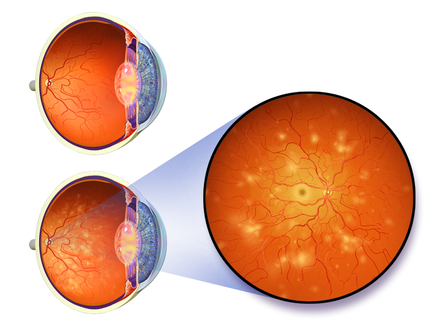
\includegraphics[scale=0.6]{images/illustration.png}
\caption{Diabetic retinopathy in comparison to a normal eye \cite{wiki}}
\label{eye}
\end{center}
\end{figure}
The primary cause of DR is that as a byproduct of the condition of diabetes, thinner blood vessels in the human body tend to form abnormal branching and thinning walls. This leads to either deteriorated blood supply to the effected areas or actual hemorrhaging. In terms of the retina, this leads to blind spots forming in the field of vision of the afflicted individual. 
To diagnose the condition, a retinal scan of the eye are taken and a scale is assigned depending on the number of abnormal vein branching, wall thickness of the blood vessels and blood stains observed. DR is categorized on a scale from 0 to 4, and examples of level 0 and 4 are shown below.

\begin{figure}[htbp]
\begin{center}
 \subfigure[Level 0 DR]{\label{reference}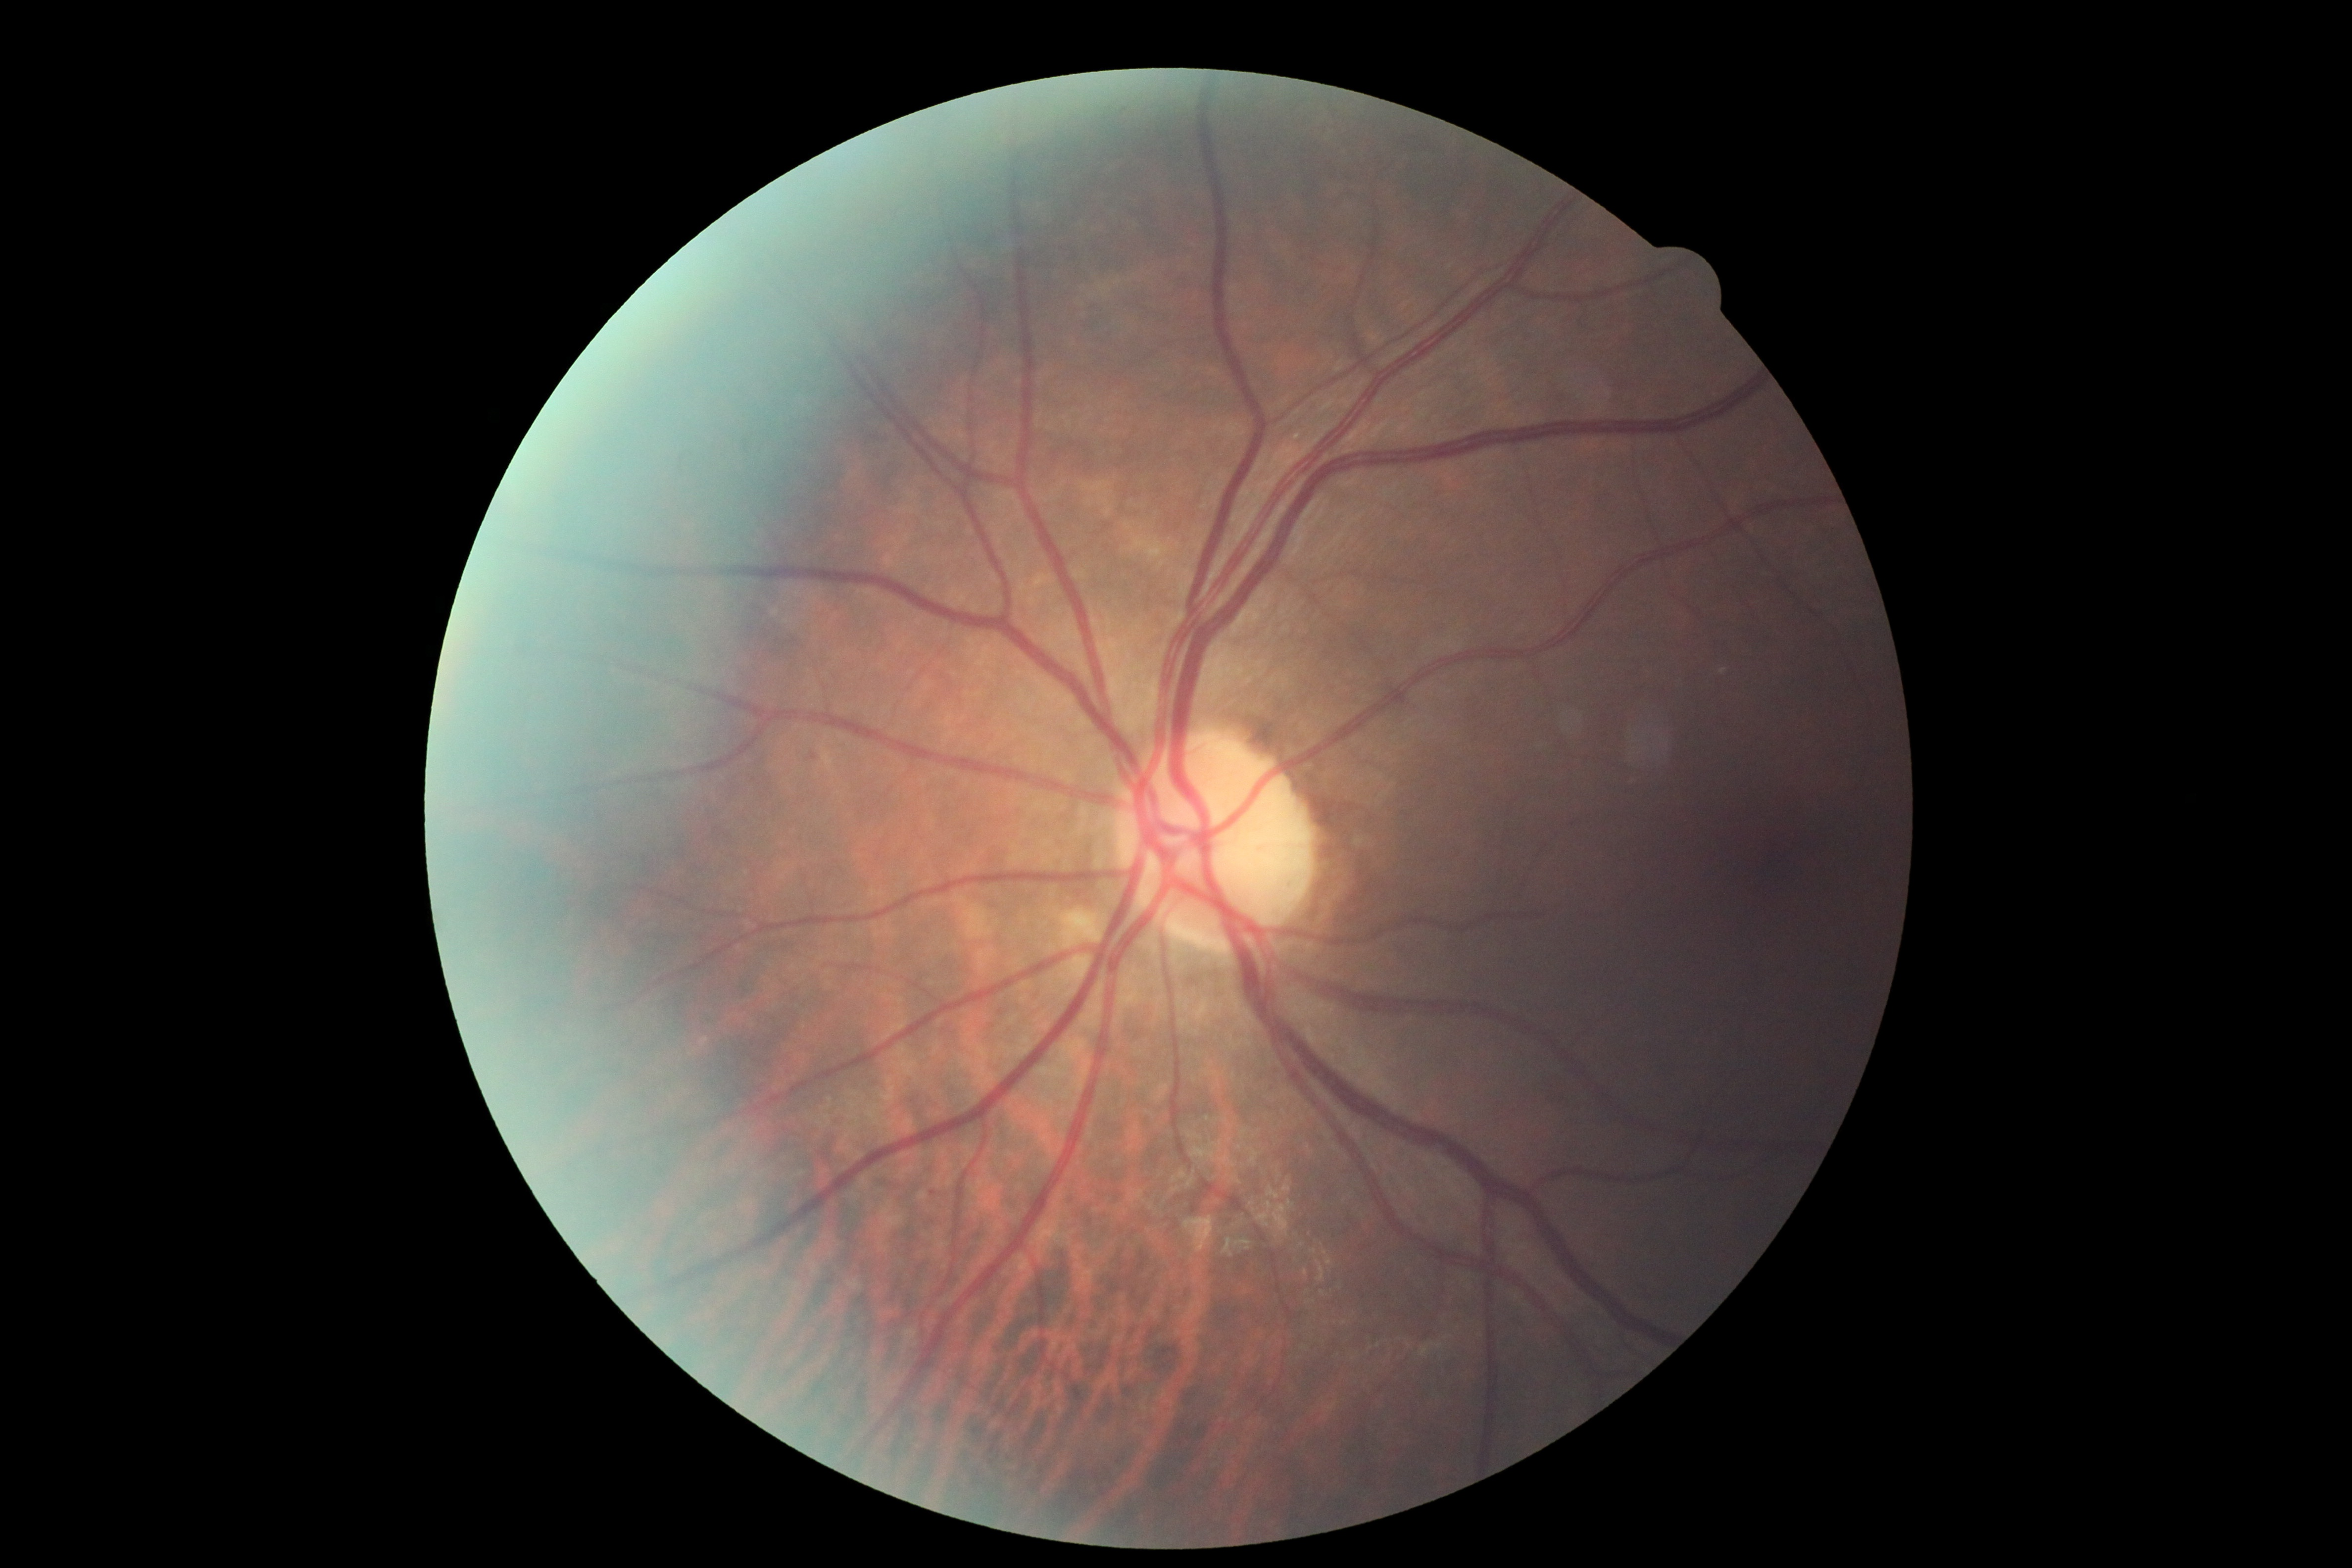
\includegraphics[scale=0.035]{images/0_Level_Example.jpeg}}
  \ \ \ \ 
\subfigure[Level 4 DR]{\label{new}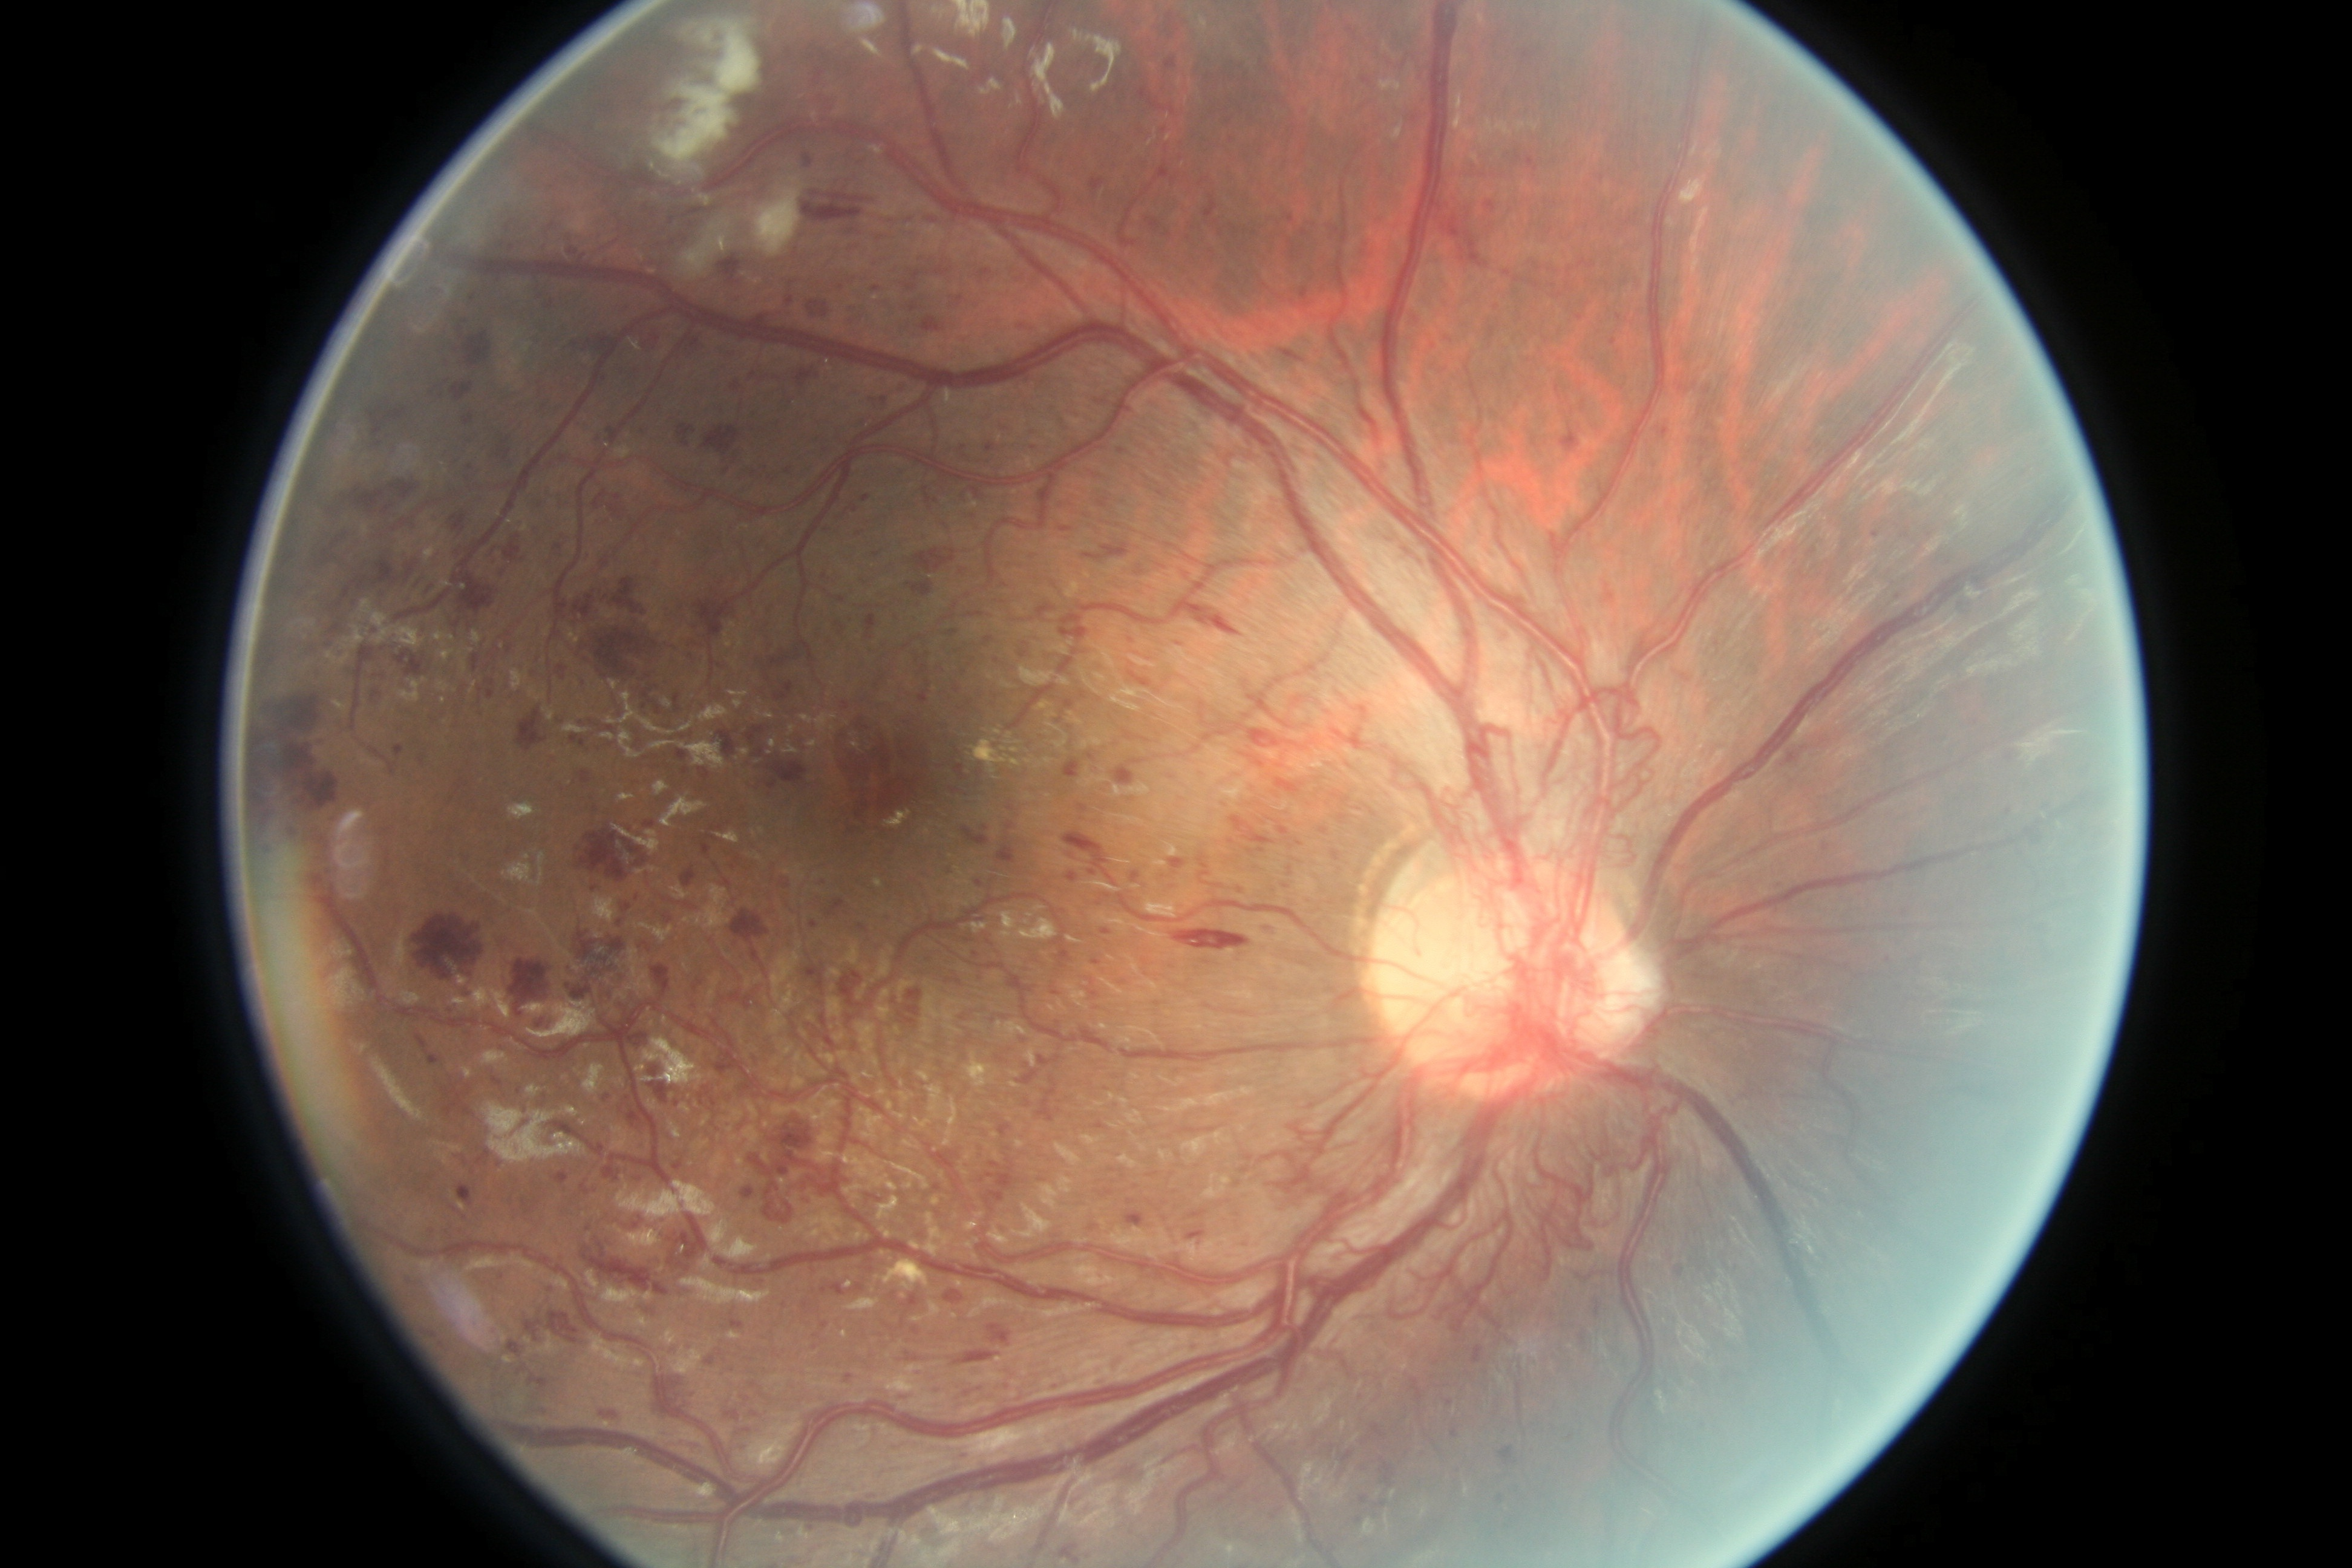
\includegraphics[scale=0.035]{images/4_Level_Example.jpeg}}
\caption{Examples of level 0 and level 4 DR}
\label{marking_image}
\end{center}
\end{figure}


\newpage
% \nocite{*}
\bibliographystyle{unsrt}
\bibliography{References}

\end{document}